\documentclass[10pt]{beamer}
\usepackage[british]{babel}
\usepackage[utf8]{inputenc}
\usepackage[T1]{fontenc}
\usepackage{hyperref}
\usetheme{Warsaw}
\usecolortheme{wolverine}
\usepackage[color,matrix,arrow]{xy}
\definecolor{Blue}{RGB}{0,0,148}
\definecolor{arancio}{RGB}{255,133,34}
\definecolor{fantasma}{RGB}{233,233,243}
\definecolor{aranciopallido}{RGB}{255,239,213}
%\useinnertheme[red]{rounded}
%\useoutertheme{infolines}
\usepackage{pdfsync}
%\renewcommand{\theequation}{\fnsymbol{\ast}}
% \usepackage[all,cmtip]{xypic}
%\usepackage{diagxy}
\usepackage[utf8]{inputenc}
\usepackage{graphicx}
\usepackage{palatino}
\usepackage{color}
%\usepackage{tikz}
\usepackage{amsfonts,amsmath,amssymb,amsthm,bbm}
\usefonttheme{professionalfonts}
\usepackage{verbatim}
\newtheorem*{conj}{Conjecture}
\newtheorem*{dfz}{Définition}
\newtheorem*{trm}{Théorème}
\date{May $23^\text{rd}, 2022$}
\title{Explaining Mathematical Proofs to Computers}
 \author[Filippo A. E. Nuccio]{Filippo Alberto Edoardo Nuccio\\ Mortarino Majno di Capriglio}
 \institute[ICJ - UJM]{Institut Camille Jordan\\
 Université de Lyon \& Université Jean Monnet de Saint-Étienne}
\begin{document} 
\frame{\titlepage}
\begin{frame}
\frametitle{What is \texttt{Lean}?}
\setlength{\tabcolsep}{8pt}
\def\arraystretch{1.5}
%\begin{center}
\begin{tabular}{ c c c  }
\centering

\includegraphics[scale=.45]{french_flag.png}&&
\includegraphics[scale=.4]{union_jack.png}\\\\
Un \textcolor{red}{assistant} de preuve&&A theorem \textcolor{Blue}{prover}\\
    % &&\\
    % Un {\textcolor{blue}vérificateur} de preuves&&A formal proof checker
\end{tabular}
%\end{center}
\end{frame}
\begin{frame}
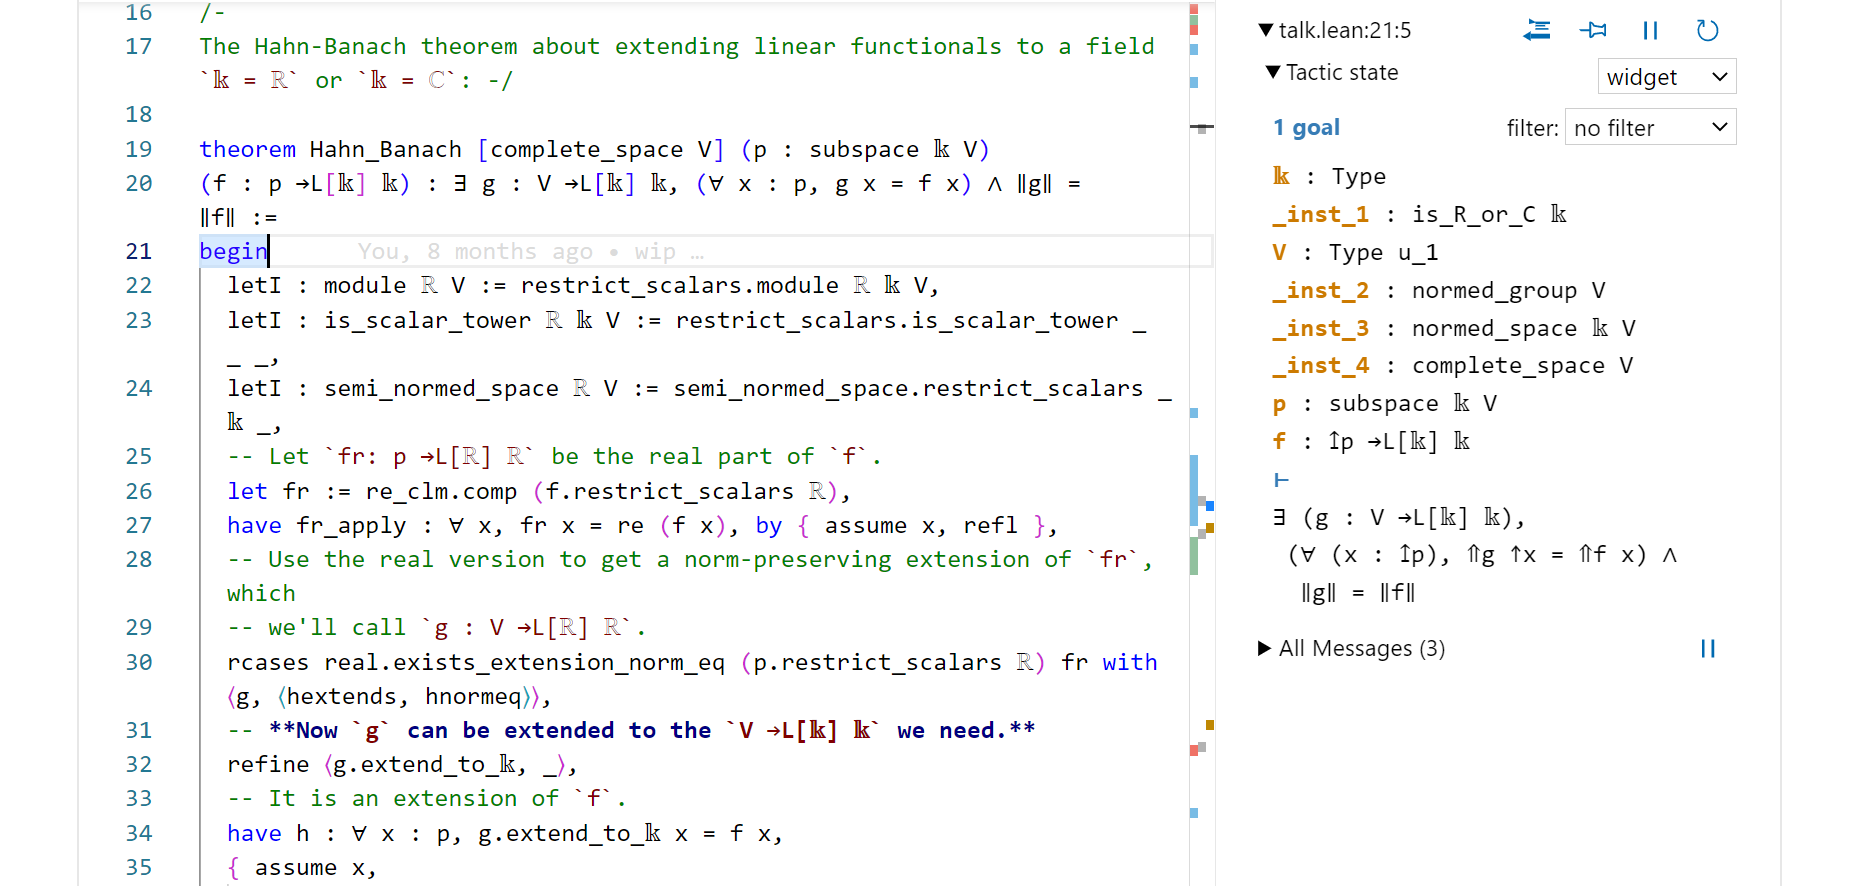
\includegraphics[trim=2.2cm 0 0 -1cm, scale = .285]{Hahn_Banach.png}
\end{frame}
\begin{frame}
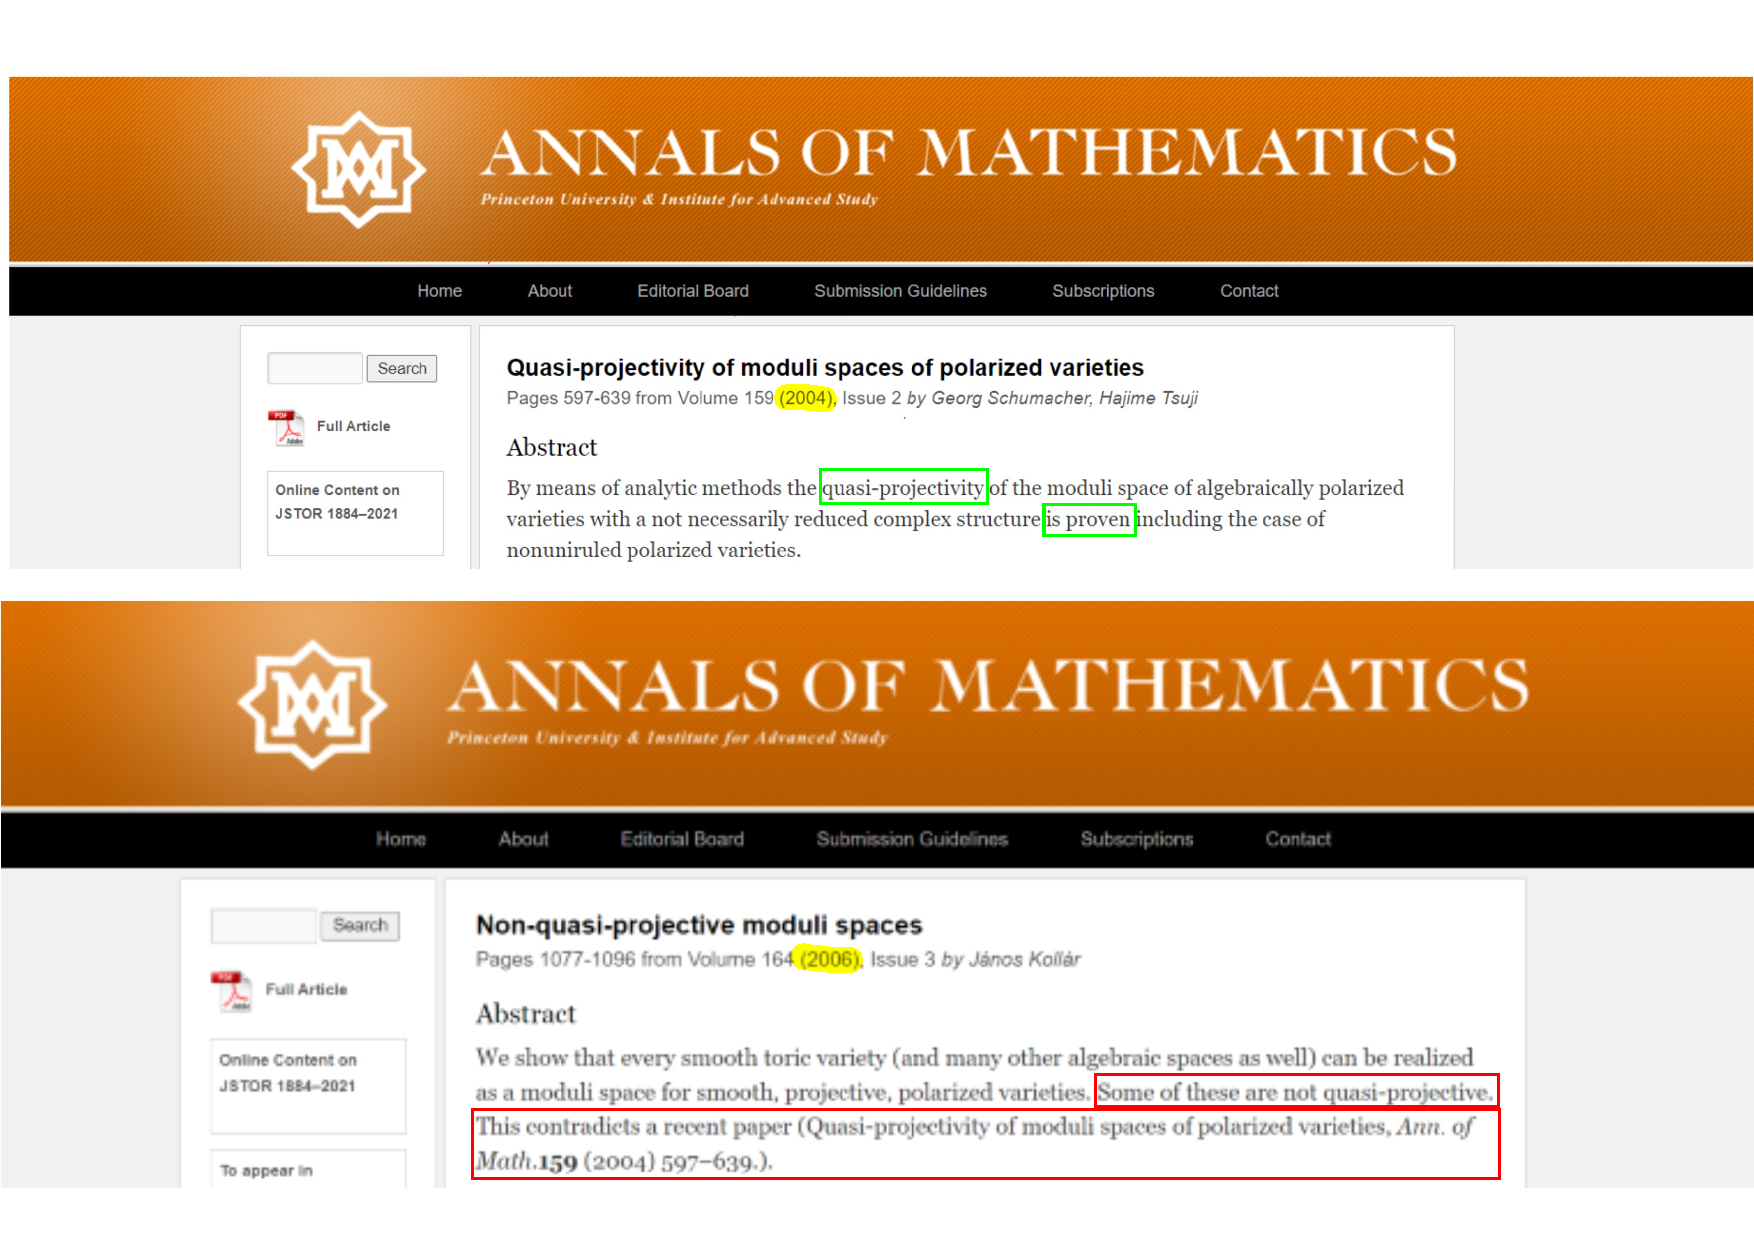
\includegraphics[trim=1.3cm 0 0 1cm, scale = .4]{Annals_Flattened.pdf}
\end{frame}
%%%%Frame: NOW TO LEAN!
\begin{frame}
\frametitle{Let's do some Lean}

\includegraphics[scale=.15]{vscode_logo.png}\hspace{1cm}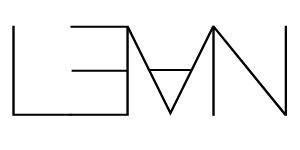
\includegraphics[trim=0 -1.45cm 5cm 5cm, scale=.5]{lean_logo.png}
\end{frame}
%%%Frame LTE
\begin{frame}
%\vspace{-.25cm}
%``The development of mathematics toward greater precision has led, as is well known, to the formalization of large tracts of it, so one can prove any theorem using nothing but a few mechanical rules. The most comprehensive formal systems that have been set up hitherto are the system of \emph{Principia Mathematica} on the one hand and the Zermelo--Fraenkel axiom system of set theory on the other.
These two systems ({\color{arancio}Principia Mathematica and Zermelo--Fraenkel}) are so comprehensive that in them all methods of proof used today in mathematics are formalized, that is, reduced to a few axioms and rules of inference. One might therefore conjecture that these axioms and rules of inference are sufficient to decide any mathematical question that can at all be formally expressed in these systems.   \only<1>{''}
\pause

It will be shown below that this is not the case.''

\vspace{.25cm}

(K.~Gödel, \emph{ On formally undecidable propositions of Principia
Mathematica and related systems}, 1931.)
\end{frame}
\begin{frame}
{\Large Liquid tensor experiment}
\only<1>{\vspace{.5cm}}
\emph{Posted\only<1-2>{\footnote{On the Xena Project blog, see \url{https://xenaproject.wordpress.com/2020/12/05/liquid-tensor-experiment/}}}, on December $5^\text{th}$, 2020}
\vspace{.5cm}

\only<1-2>
{I \textcolor{arancio}{[Peter Scholze]} want to propose a challenge: Formalise the proof of the following theorem.

\begin{theorem}[Clausen--S.] Let $0<p'<p\leq 1$ be real numbers, let $S$ be a profinite set, and let $V$ be a $p$-Banach space. Let $\mathcal M_{p'}(S)$ be the space of $p'$-measures on $S$. Then
\[
\mathrm{Ext}^i_{\mathrm{Cond}(\mathrm{Ab})}(\mathcal M_{p'}(S),V)=0
\]
for $i\geq 1$.
\end{theorem}}
\pause
\only<2>
{\vspace{.75cm}
Why do I want a formalization?}
\pause
\only<3>
{\begin{itemize}
\item \dots
\item ~[\dots] In the end, we were able to get an argument pinned down on paper, but I think nobody else has dared to look at the details of this, and so I still have some small lingering doubts.
\item ~[\dots] I think the theorem is of utmost foundational importance, so being 99.9\% sure is not enough.
\item I have occasionally been able to be very persuasive even with wrong arguments. \footnote{Fun fact: In the selection exams for the international math olympiad, twice I got full points for a wrong solution. Later, I once had a full proof of the weight-monodromy conjecture that passed the judgment of some top mathematicians, but then it turned out to contain a fatal mistake.}
\item I think this may be my most important theorem to date [\dots]. Better be sure it’s correct\dots
\end{itemize}}
\end{frame}
\begin{frame}
{\Large Liquid tensor experiment}
\emph{Posted\footnote{Voir \url{https://xenaproject.wordpress.com/2021/06/05/half-a-year-of-the-liquid-tensor-experiment-amazing-developments/}} on June 5, 2021}
\vspace{.5cm}

Exactly half a year ago I wrote the Liquid Tensor Experiment blog post, challenging the formalization of a difficult foundational theorem from my Analytic Geometry lecture notes on joint work with Dustin Clausen. While this challenge has not been completed yet, I am excited to announce that \textcolor{arancio}{the Experiment has verified the entire part of the argument that I was unsure about}. I find it absolutely insane that \textcolor{arancio}{interactive proof assistants are now at the level that within a very reasonable time span they can formally verify difficult original research}. Congratulations to everyone involved in the formalization!!
\end{frame}

\end{document}